%%%%%%%%%%%%%%%%%%%%%%%%%%%%%%%%%%%%%%%%%
% Short Sectioned Assignment
% LaTeX Template
% Version 1.0 (5/5/12)
%
% This template has been downloaded from:
% http://www.LaTeXTemplates.com
%
% Original author:
% Frits Wenneker (http://www.howtotex.com)
%
% License:
% CC BY-NC-SA 3.0 (http://creativecommons.org/licenses/by-nc-sa/3.0/)
%
%%%%%%%%%%%%%%%%%%%%%%%%%%%%%%%%%%%%%%%%%

%----------------------------------------------------------------------------------------
%	PACKAGES AND OTHER DOCUMENT CONFIGURATIONS
%----------------------------------------------------------------------------------------

\documentclass[paper=a4, fontsize=11pt]{scrartcl} % A4 paper and 11pt font size

\usepackage[T1]{fontenc} % Use 8-bit encoding that has 256 glyphs
\usepackage{fourier} % Use the Adobe Utopia font for the document - comment this line to return to the LaTeX default
\usepackage[english]{babel} % English language/hyphenation
\usepackage{amsmath,amsfonts,amsthm} % Math packages
\usepackage[utf8]{inputenc}
\usepackage{graphicx}
\usepackage{tabularx}
\usepackage{longtable}
\usepackage{threeparttable}
\usepackage{booktabs}
\usepackage{listings}
\usepackage[numbered,autolinebreaks,useliterate]{mcode}
\usepackage{float}
\usepackage{algpseudocode}
\usepackage[tight,footnotesize]{subfigure}
\usepackage{cprotect}


\usepackage{lipsum} % Used for inserting dummy 'Lorem ipsum' text into the template

\usepackage{sectsty} % Allows customizing section commands
\allsectionsfont{\centering \normalfont\scshape} % Make all sections centered, the default font and small caps

\usepackage{fancyhdr} % Custom headers and footers
\pagestyle{fancyplain} % Makes all pages in the document conform to the custom headers and footers
\fancyhead{} % No page header - if you want one, create it in the same way as the footers below
\fancyfoot[L]{} % Empty left footer
\fancyfoot[C]{} % Empty center footer
\fancyfoot[R]{\thepage} % Page numbering for right footer
\renewcommand{\headrulewidth}{0pt} % Remove header underlines
\renewcommand{\footrulewidth}{0pt} % Remove footer underlines
\setlength{\headheight}{13.6pt} % Customize the height of the header

\numberwithin{equation}{section} % Number equations within sections (i.e. 1.1, 1.2, 2.1, 2.2 instead of 1, 2, 3, 4)
\numberwithin{figure}{section} % Number figures within sections (i.e. 1.1, 1.2, 2.1, 2.2 instead of 1, 2, 3, 4)
\numberwithin{table}{section} % Number tables within sections (i.e. 1.1, 1.2, 2.1, 2.2 instead of 1, 2, 3, 4)

\setlength\parindent{0pt} % Removes all indentation from paragraphs - comment this line for an assignment with lots of text

% new command for short vertical space
\newcommand{\vertbreak}{\vspace{1.75 mm}}

% define "struts", as suggested by Claudio Beccari in
%    a piece in TeX and TUG News, Vol. 2, 1993.
\newcommand\Tstrut{\rule{0pt}{2.6ex}}         % = `top' strut
\newcommand\Bstrut{\rule[-0.9ex]{0pt}{0pt}}   % = `bottom' strut

%----------------------------------------------------------------------------------------
%	TITLE SECTION
%----------------------------------------------------------------------------------------

\newcommand{\horrule}[1]{\rule{\linewidth}{#1}} % Create horizontal rule command with 1 argument of height

\title{	
\normalfont \normalsize 
\textsc{Faculdade de Engenharia da Universidade do Porto} \\ [25pt] % Your university, school and/or department name(s)
\horrule{0.5pt} \\[0.4cm] % Thin top horizontal rule
\LARGE Machnine Learning (PDEEC0049 : 15-782PP)\\ \Large Homework 5 \\ % The assignment title
\horrule{2pt} \\[0.5cm] % Thick bottom horizontal rule
}

\author{António Damião das Neves Rodrigues (200400437 : 700098386)} % Your name

\date{\normalsize\today} % Today's date or a custom date

\begin{document}

\maketitle % Print the title

\section{Problem 1}

\subsection{}
\label{subsec:1-1}

\begin{figure}[h!]

    \centering
    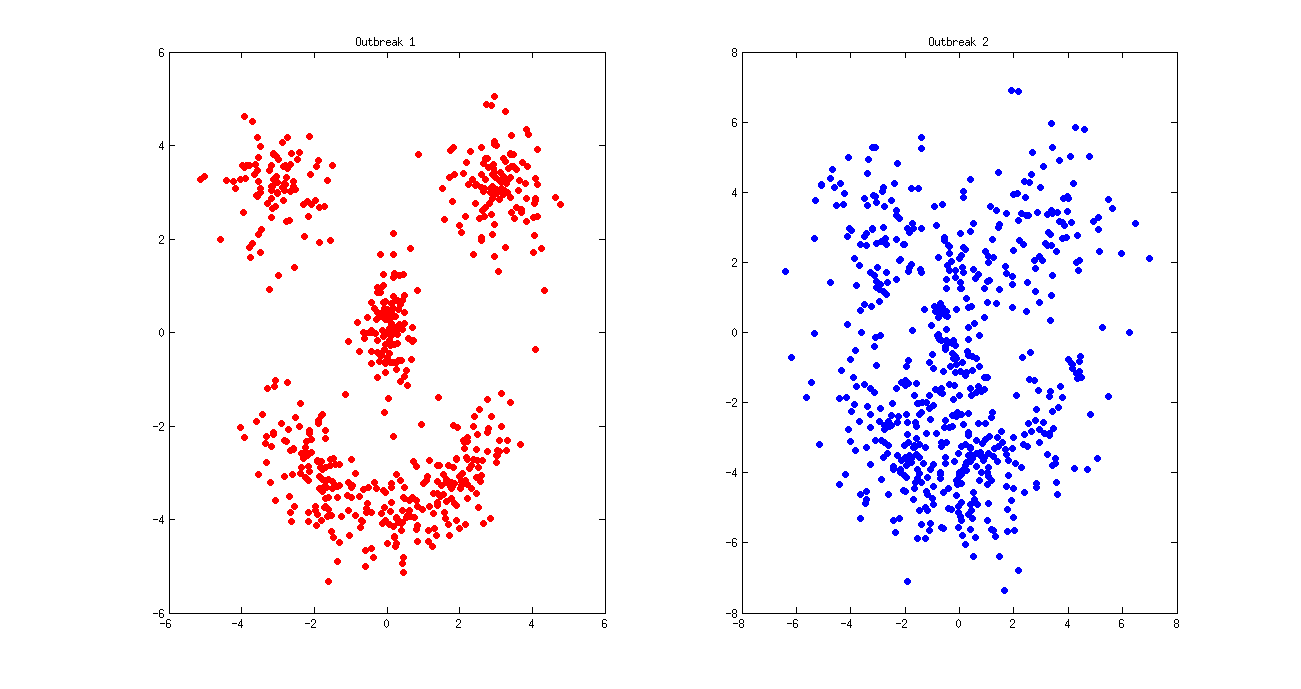
\includegraphics[width=1.00\textwidth]{figures/outbreak.png}
    \caption{Geographical spread of infected computers, for the two virus 
            outbreaks.}
    \label{fig:1-1}

\end{figure}

\subsection{}
\label{subsec:1-2}

Use the MATLAB code given as attachment (\verb+problem1+ folder) files 
\verb+kmeans.m+ and \verb+em.m+ for implementation details. Follow the comments 
on the code for details and reasoning. The MATLAB file \verb+problem1.m+ was 
used for testing the implementations (in that file you may choose the 
values of the dataset and $K$ to test).\vertbreak

Figure~\ref{fig:1-2} shows the partial result of running \verb+problem1_2.m+, for 
$K = 4$ and $K = 6$, for the \verb+joker1+ dataset. Notice that the final cluster 
centers of K-Means are used as the initial means for the Gaussiam Mixture Model 
(GMM), before running the Expected Maximization (EM) algorithm for GMMs.

\begin{figure}[H]
    \centering

    \subfigure[]{
        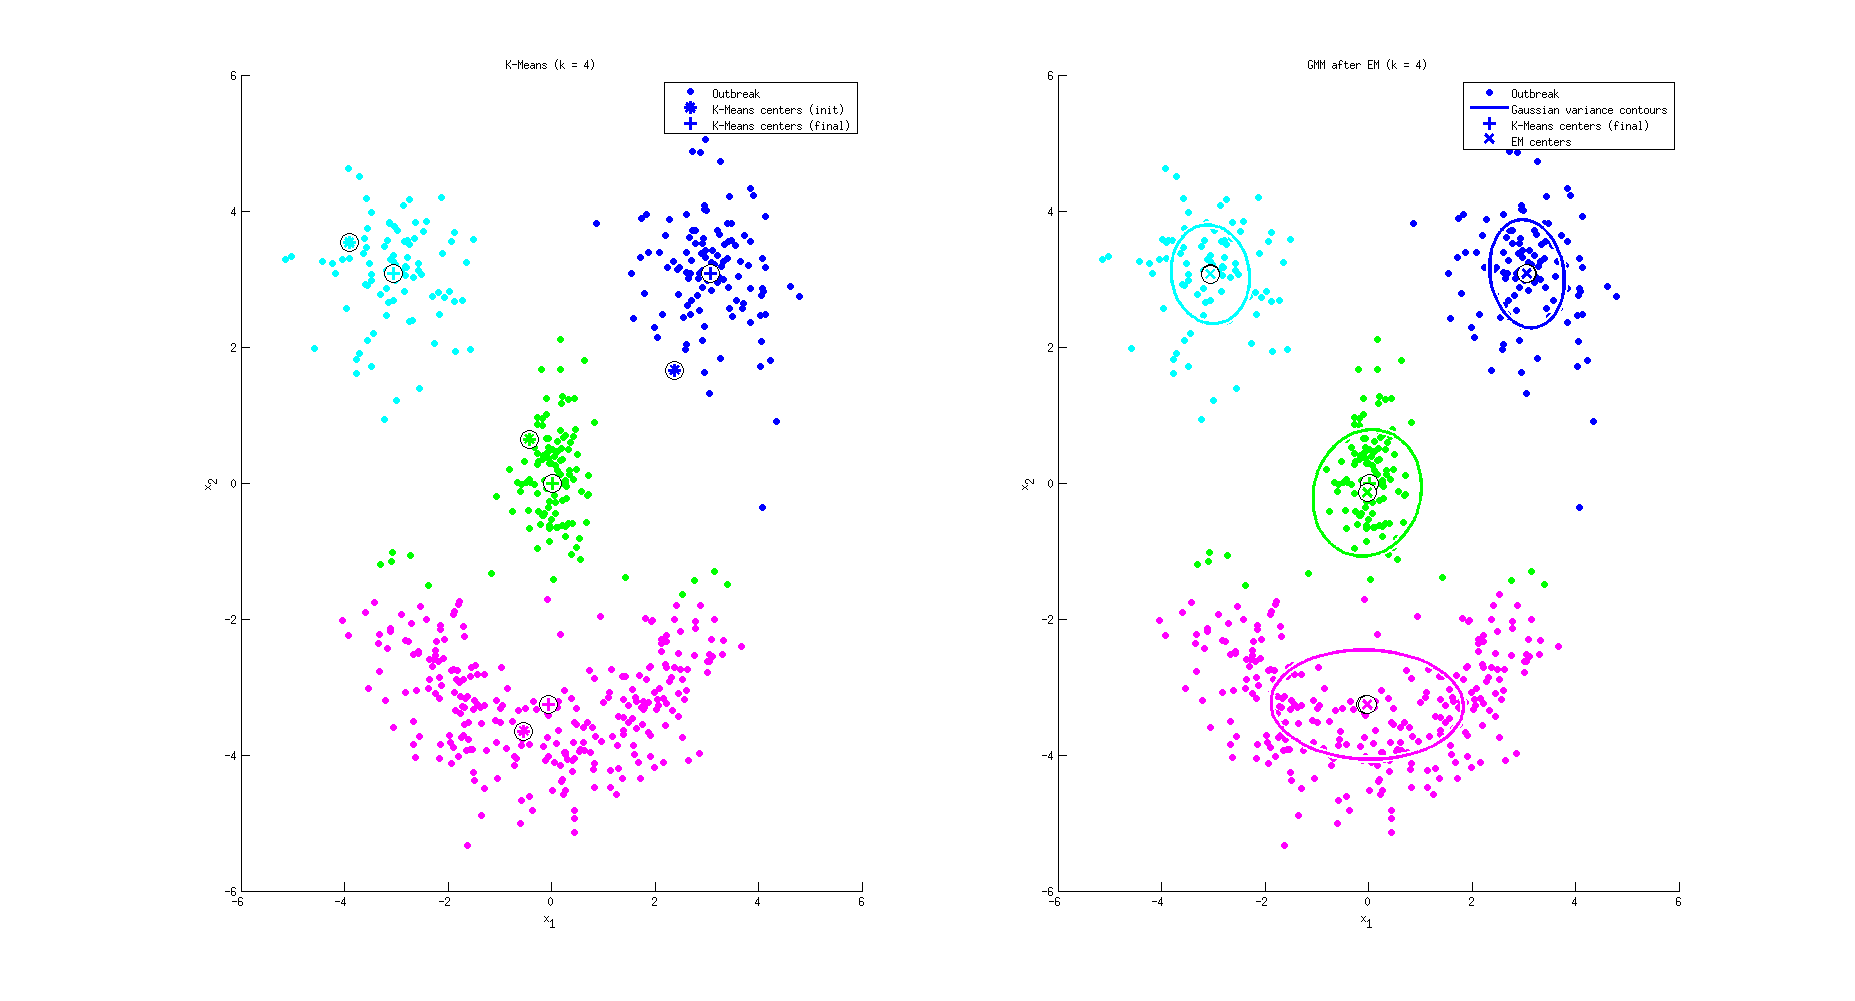
\includegraphics[width=1.00\textwidth] {figures/k4.png}
        \label{subfig:1-2-k6}
    }

    \subfigure[]{
        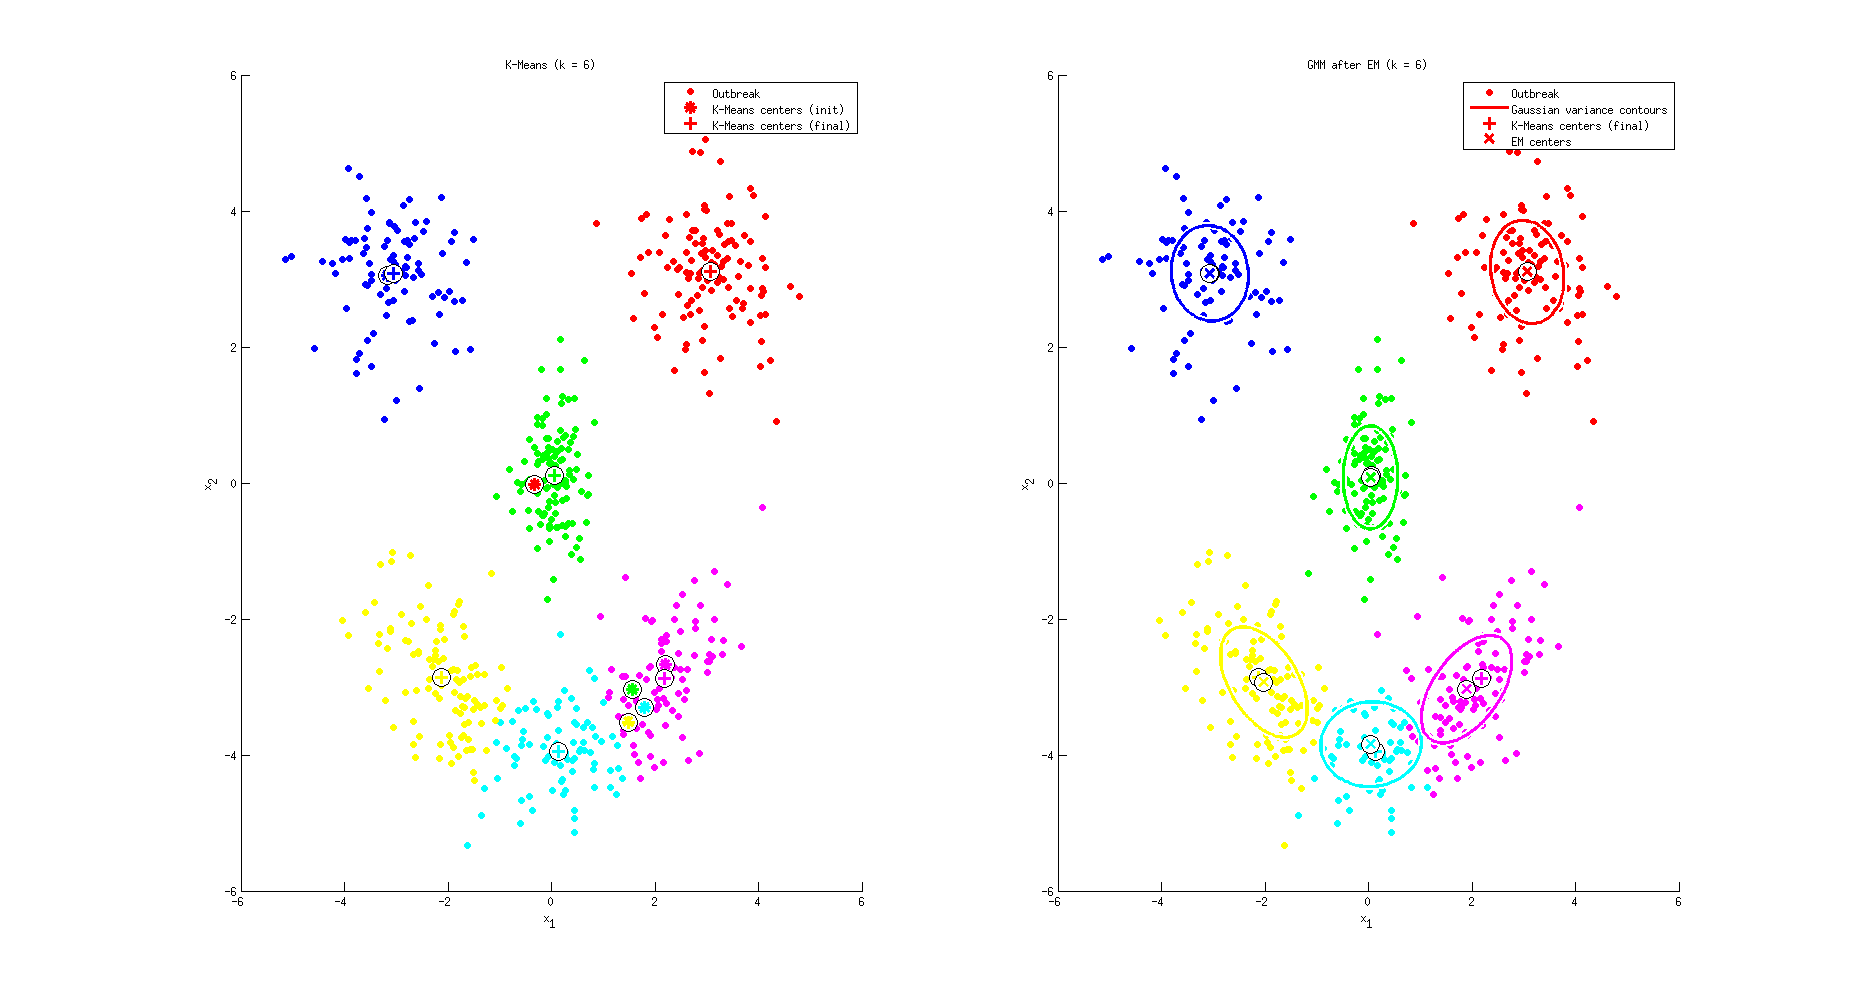
\includegraphics[width=1.00\textwidth] {figures/k6.png}
        \label{subfig:1-2-k4}
    }

    \cprotect\caption{Clustering after running K-Means and the EM algorithm 
        for GMMs, for the \verb+joker1+ dataset, $K = 4$ (a) and 
        $K = 6$ (b).}
    \label{fig:1-2}

\end{figure}

\subsection{}
\label{subsec:1-3}

Use the MATLAB code given as attachment (\verb+problem1+ folder) files 
\verb+problem1_3.m+ and \verb+cluster.m+ for implementation details. Follow the 
comments on the code for details and reasoning. The MATLAB 
file \verb+problem1_3.m+ was used for testing the implementations.\vertbreak

The script \verb+problem1_3.m+ generates a series of subplot groups, for each 
$\{K,$\verb+joker*+$\}$ combination. See Figure~\ref{fig:1-3} for an example.

\begin{figure}[h!]

    \centering
    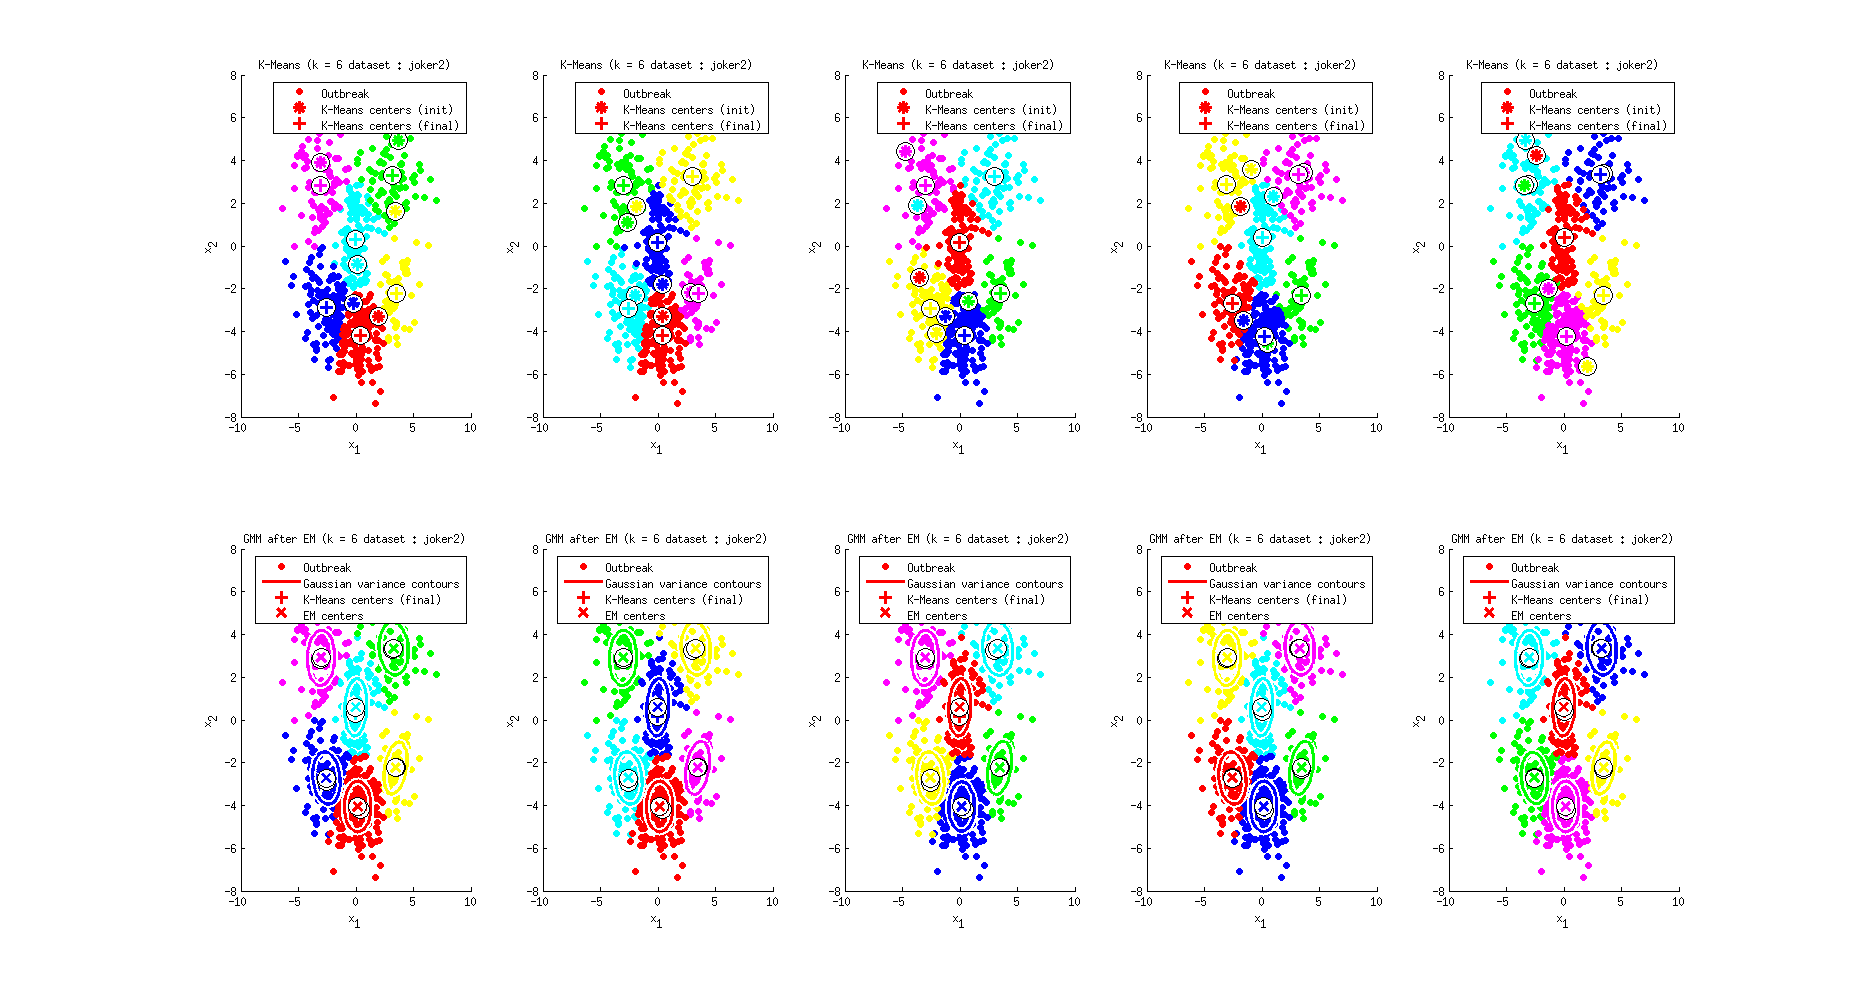
\includegraphics[width=1.00\textwidth]{figures/1-3.png}
    \cprotect\caption{Example of output of the \verb+problem1_3.m+ MATLAB script, for 
        $K = 6$, dataset \verb+joker2+. Each column corresponds to a different 
        group of initial centers, the final cluster centers of K-Means are used as 
        the initial means for the GMM approach.}
    \label{fig:1-3}

\end{figure}

\section{Problem 2}

Use the MATLAB code given as attachment (\verb+problem2+ folder) files 
\verb+hmmTest.m+ for implementation details. Follow the comments on the code 
for details and reasoning.\vertbreak

Table~\ref{tab:2-1} shows the computed probabilities for the given sequence, 
using both forward and backward algorithms (both compute the same value).

\begin{table}[H]
\begin{center}
    \small
        \begin{tabularx}{0.35\textwidth}{ c | c }
            %\hline
            Algorithm   & $P(x|M)$          \\ [0.5ex]
            \hline
            Forward     & 0.094205886087188 \\ [0.5ex]
            %\hline
            Backward    & 0.094205886087188 \\ [0.5ex]
        \end{tabularx}
    \caption{Computed probabilities for the sequence of length 10 in Problem 
            2, given the provided Hidden Markov Model $M$, using both forward 
            and backward algorithms.}
    \label{tab:2-1}
    \end{center}
\end{table}

\section{Problem 3}

\subsection{}
\label{subsec:3-1}

\textbf{Assumptions:}

\begin{enumerate}

    \item The WSN is formed by a $N \times N$ square matrix of nodes $W$. 
            Therefore, there are $N^2$ nodes in the WSN and each position 
            $(i,j)$ of $W$ is occupied by a wireless node.
    \item When a node in the WSN transmits a message, all other nodes receive 
            the message, i.e. messages are broadcast.
    \item All nodes have memory capabilities to store the state of the matrix $W$, 
            in which each position $(i,j)$ of $W$ holds the value(s) for each 
            variable $v$ sensed by the WSN node at position $(i,j)$.
    \item A WSN node can transmit any one or more types of data it knows in one 
            message or a function of this data.
    \item Every node is aware of its $(i,j)$ coordinates within $W$.
    \item All nodes are aware of their inclusion in a $N \times N$ square 
            matrix $W$, with each position accessed via coordinates $(i,j)$.
    \item Among the $N^2$ nodes of the WSN, there is a master node $M$, with 
            the capability of starting network procedures.
    \item In the following descriptions, the indexing of arrays starts at `0', 
            e.g. the first element of an array $F$ would be $F[0]$.

\end{enumerate}

\textbf{Algorithm:}

\begin{algorithmic}[1]

\State Compute factors of $N$. Store them in ascending order in $F = \{1, ..., N\}$.
\State $k \leftarrow 1$
\State $T \leftarrow M$

\For{$\frac{N}{F[k]} \ge S$}

\State Divide $W$ in $F[k]^2$ squares of side $\frac{N}{F[k]}$.

\ForAll{unvisited squares of side $\frac{N}{F[k]}$}

\State Node $T$ sends message with format $\{(i,j); \text{value}; (i',j'\}$. 
        The value $(i',j')$ is a random position within one of the unvisited 
        $F[k]^2$ squares, excluding $(i,j)$ positions already known in $W$.

\State All nodes update the matrix $W$ with the contents of the message from 
        node $T$.

\State $T \leftarrow \text{node}(i',j')$

\EndFor

\State Determine the min. and max. values of the known nodes in $W$, 
        $W_{min}$ and $W_{max}$.
\State Set all unknown $(i,j)$ slots of $W$ to $W_{min}$.
\State Save new positions $(i,j)$ of the local maxima (peaks) of $W$ in the 
        \textbf{means} array $U$.

\State $k \leftarrow k + 1$
\State $T \leftarrow$ any unvisited node in $W$

\EndFor

\ForAll{positions $(i,j)$ in $U$} 

\State From the $K^2 - 1$ neighbor positions of $U_n$, those which are unknown 
        in matrix $W$ send messages in the format $\{(i,j); \text{value}\}$.

\State All nodes update the matrix $W$ with the contents of the message from 
        the neighbor nodes.

\EndFor

\State Save new positions $(i,j)$ of the local maxima (peaks) of $W$ in the 
        \textbf{means} array $U$.

\end{algorithmic}\vertbreak

\textbf{Explanation:}\vertbreak

The first part of the algorithm (lines 4 to 16) consists in sampling the 
sensor values in a distributed manner. The precision of the sampling --- and the 
number of exchanged messages --- can be tuned via the $S$ parameter (the 
minimum side size of the square partitions to apply in $N \times N$ matrix of sensors).
With $S = 1$, we would get the complete knowledge of the dataset, i.e. $N^2$ 
exchanged messages.\vertbreak

The second part (lines 17 to 21) attempts to gather more knowledge around the 
pre-selected means $U$ of the matrix $W$, by retrieving the values of its 
neighbors. The neighborhood structure is a square of size $K^2$ (also tunable), 
centered around each element of $U$.\vertbreak

After this sampling phase, the idea would be to use EM for GMMs in the regular 
way, using the elements of $U$ as the initial means, to determine the remaining 
parameters of the GMM.\vertbreak

The cost in messages of the algorithm would be: $(\frac{N}{S})^2 + 
((\text{size}(U) \times (K^2 - 1)) - A)$. Note that the second additive term varies with $A$, 
the number of neighbors of the nodes in $U$ already known at the time of running the second phase
 of the algorithm. E.g. for $S = 1$, we would know the entire dataset after the first phase of 
the algorithm, so the values of all $K^2 - 1$ neighbors within the \verb+for+ cycle in line 17 
would be known, therefore $(\text{size}(U) \times (K^2 - 1) - A) = 0$, so, in the 
worst case, this method would also cost $N^2$ messages.

\subsection{}
\label{subsec:3-2}

Regarding the algorithm presented in Section~\ref{subsec:3-1}, the knowledge of 
a global maximum would allow it to start similarly to its second part: 
(1) determine one of initial means $U_n$ (a peak) and (2) the $K^2 - 1$ 
neighborhood of $U_n$.\vertbreak

As the proposed algorithm already tries to gather $K^2 - 1$ values around or 
near that peak, that knowledge would not contribute to reduce the number of 
exchanged messages.

\bibliographystyle{plain}
\bibliography{hw5.bib}

\end{document}
